\documentclass[fleqn]{article}
\usepackage[margin=1in]{geometry}
\usepackage[nodisplayskipstretch]{setspace}
\usepackage{amsmath, nccmath, bm}
\usepackage{amssymb}
\usepackage{enumitem}
\usepackage{graphicx}
\usepackage{float}
\usepackage{listings}
\usepackage{hyperref}
\usepackage[svgnames]{xcolor}
\graphicspath{{./images}}

\hypersetup{
    colorlinks=true,
    linkcolor=black,
    filecolor=black,      
    urlcolor=blue
    }

\newcommand{\zerodisplayskip}{
	\setlength{\abovedisplayskip}{0pt}%
	\setlength{\belowdisplayskip}{0pt}%
	\setlength{\abovedisplayshortskip}{0pt}%
	\setlength{\belowdisplayshortskip}{0pt}%
	\setlength{\mathindent}{0pt}}
	
\definecolor{vgreen}{RGB}{104,180,104}
\definecolor{vblue}{RGB}{49,49,255}
\definecolor{vorange}{RGB}{255,143,102}

\lstdefinestyle{verilog-style}
{
    language=Verilog,
    basicstyle=\small\ttfamily,
    keywordstyle=\color{vblue},
    identifierstyle=\color{black},
    commentstyle=\color{vgreen},
    numbers=left,
    numberstyle=\tiny\color{black},
    numbersep=10pt,
    tabsize=8,
    moredelim=*[s][\colorIndex]{[}{]},
    literate=*{:}{:}1
}

\lstset{style={verilog-style},showstringspaces=false}

\makeatletter
\newcommand*\@lbracket{[}
\newcommand*\@rbracket{]}
\newcommand*\@colon{:}
\newcommand*\colorIndex{%
    \edef\@temp{\the\lst@token}%
    \ifx\@temp\@lbracket \color{black}%
    \else\ifx\@temp\@rbracket \color{black}%
    \else\ifx\@temp\@colon \color{black}%
    \else \color{vorange}%
    \fi\fi\fi
}
\makeatother

\newcommand{\code}[1]{%
	\colorbox{Gainsboro}{\texttt{#1}}%
}

\title{Homework 2}
\author{Owen Sowatzke}
\date{February 24, 2025}

\begin{document}

	\offinterlineskip
	\setlength{\lineskip}{12pt}
	\zerodisplayskip
	\maketitle
	
	\begin{enumerate}
		\item Based on the figures below mention which figure depicts the mode of operation and briefly describe its operation in terms of the figure.
		
		\begin{enumerate}
		
			\item Figure \ref{fig::mode_of_operations_part_a} depicts the cutoff region. In this region, there is no channel between the source and drain. The n+ doping around the source and drain forms reversed-biased PN junctions with the p-type body, preventing current from flowing. As such, the current between the source and drain ($I_{D}$) is approximately zero.
			
			\begin{figure}[H]				
				\centerline{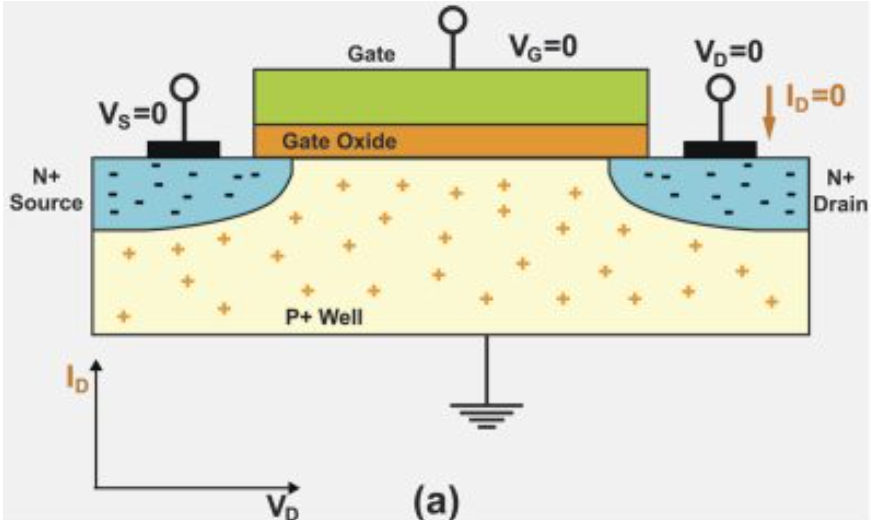
\includegraphics[width=0.5\textwidth]{mode_of_operations_part_a.png}}
				\caption{CMOS Transistor in Cutoff Region}
				\label{fig::mode_of_operations_part_a}
			\end{figure}
		
			\item Figure \ref{fig::mode_of_operations_part_b} depicts the resistive region. In this region, the positive gate charge attracts negative charge from the p-type body, forming a n-channel (inversion region). Between, the p and n-type regions, the drift and diffusion currents counteract to form a depletion zone. Current cannot flow through the n-channel without a potential difference between drain and source. When this potential exists, electrons flow from source to drain, creating a current from the drain to the source. For small potential difference (small values of $V_D$), the current grows linearly with applied voltage, hence the naming of this region.
			
			% The diffusion current causes negative charge to form in the p-type body and positive charge to form in the n-type body. This eventually leads to an electric field and in turn a drift current, which prevents the movement of additional charged.
			
			\begin{figure}[H]				
				\centerline{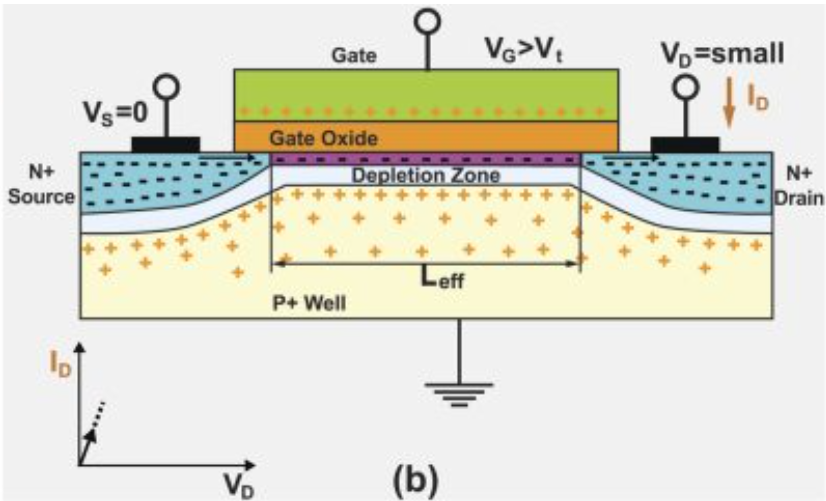
\includegraphics[width=0.5\textwidth]{mode_of_operations_part_b.png}}
				\caption{CMOS Transistor in Resistive Region}
				\label{fig::mode_of_operations_part_b}
			\end{figure}
			
			\item Figure \ref{fig::mode_of_operations_part_c} depicts the pinch-off point (start of the saturation region). Here the gate to drain voltage ($V_{gd}$) is exactly equal to the threshold voltage ($V_th$). $V_{gd}$ must be greater than the $V_{th}$ to form an inversion layer at the drain. Thus, the inversion layer and channel disappear at the drain forming what is known at the pinch-off point. Beyond this point, the drain-source current saturates at $I_{D_{SAT}}$.  
						
			% \item Figure \ref{fig::mode_of_operations_part_c} depicts the start of the saturation region. Here the channel is being pinched off at the drain because the gate to drain voltage ($V_{gd}$) falls below the threshold voltage ($V_t$). This causes the region of the channel near the drain to no longer be inverted. However, the potential difference still accelerates the electrons from source to drain. As we further increase $V_{ds}$, the drain to source current $I_{D}$ saturates at a value of $I_{D_{sat}}$.
			
			\begin{figure}[H]				
				\centerline{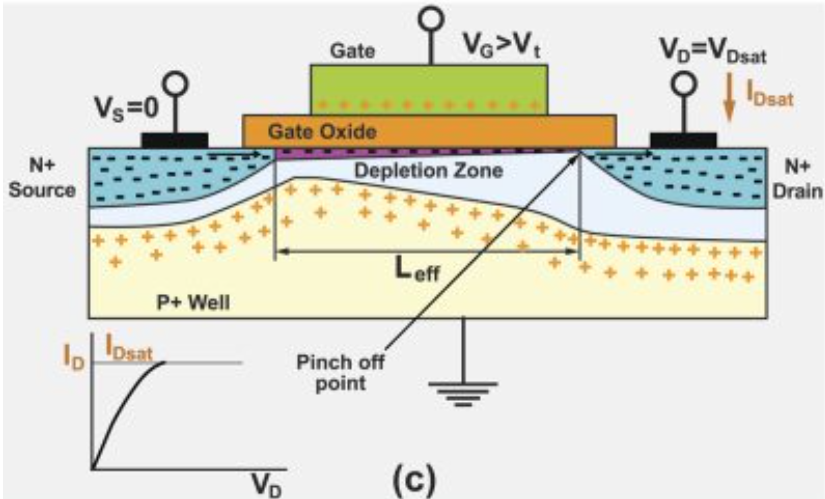
\includegraphics[width=0.5\textwidth]{mode_of_operations_part_c.png}}
				\caption{CMOS Transistor in Saturation Region }
				\label{fig::mode_of_operations_part_c}
			\end{figure}
		
			\item Figure \ref{fig::mode_of_operations_part_d} depicts the saturation region. At this point, the gate to source voltage ($V_{gs}$) is below the threshold voltage ($V_{th}$), which prevents an inversion layer from forming at the drain. Additionally, when $V_{D} > V_{D_{SAT}}$, the pinch-off point moves towards the source reducing the effective channel length, $L_{eff}$. Even though there is no channel, electrons are propelled from the channel to the drain via an electric field. At this point, the drain-source current saturates at $I_{D_{SAT}}$. 
			
			\begin{figure}[H]				
				\centerline{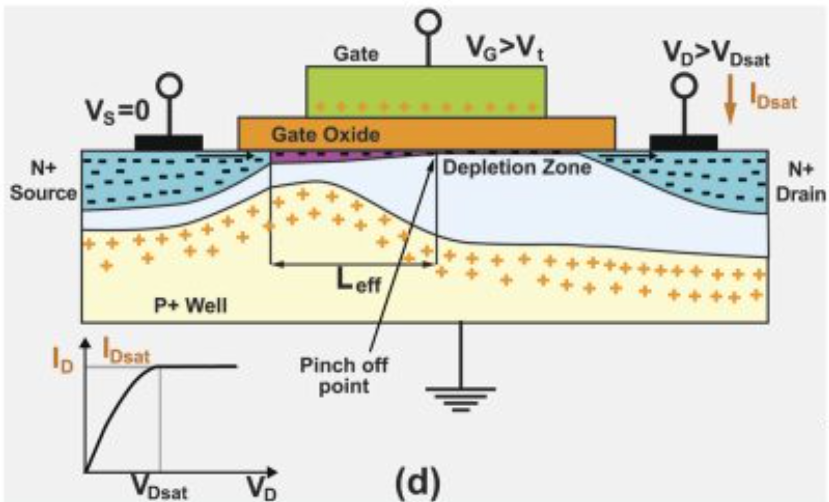
\includegraphics[width=0.5\textwidth]{mode_of_operations_part_d.png}}
				\caption{CMOS Transistor in Saturation Region}
				\label{fig::mode_of_operations_part_d}
			\end{figure}
			
		\end{enumerate}
		
		\item Describe the differences in the I-V characteristics of NMOS and PMOS transistors. How does mobility ($\mu$) affect the drain current ($I_D$) in both cases? Why must PMOS transistors be wider than NMOS to provide the same current? Support your answer with relevant equations.
		
		The IV characteristics of NMOS and PMOS transistors are shown in Figure \ref{fig::iv_characteristics_nmos} and Figure \ref{fig::iv_characteristics_pmos} respectively.
		
		\begin{figure}[H]				
			\centerline{\fbox{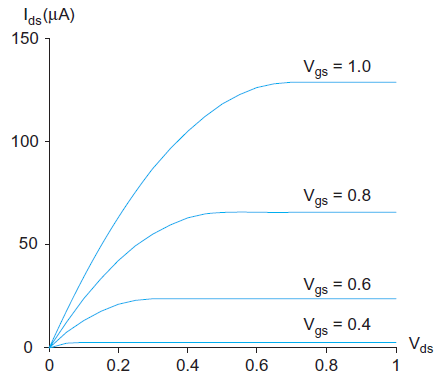
\includegraphics[width=0.5\textwidth]{iv_characteristics_nmos.png}}}
			\caption{IV Characteristic of an NMOS Transistor}
			\label{fig::iv_characteristics_nmos}
		\end{figure}
		
		\begin{figure}[H]				
			\centerline{\fbox{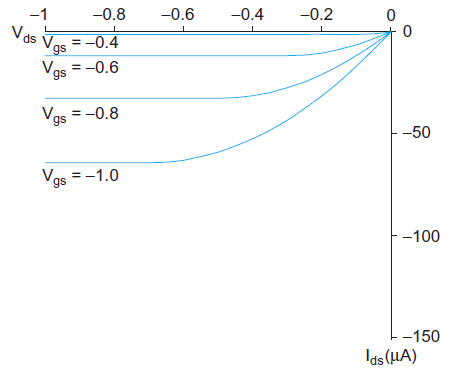
\includegraphics[width=0.5\textwidth]{iv_characteristics_pmos.png}}}
			\caption{IV Characteristic of a PMOS Transistor}
			\label{fig::iv_characteristics_pmos}
		\end{figure}
		
		For PMOS transistors, the polarities of all voltages and currents are reversed. The transistor turns on for $V_{gs} < V_t$  (or when the gate is at a lower voltage than the source). The drain current ($I_D$) is also negative for PMOS transistors because positive carriers (holes) are flowing from source to drain. The current between the source and drain also increases as the drain-source voltage ($V_{ds}$) becomes more negative.
		
		For NMOS transistors:
		
		\begin{equation*}
			I_{ds} = \begin{cases}
				0 & V_{gs} < V_t \\
				\beta_n\left(V_{gs}-V_t-\frac{V_{ds}}{2}\right)V_{ds} & V_{ds} < V_{dsat} \\
				\frac{\beta_n}{2}(V_{gs}-V_t)^2 & V_{ds} > V_{dsat}
			\end{cases}
		\end{equation*}
		
		For PMOS transistors:
		
		\begin{equation*}
			I_{ds} = \begin{cases}
				0 & V_{gs} > V_t \\
				-\beta_p\left(V_{gs}-V_t-\frac{V_{ds}}{2}\right)V_{ds} & V_{ds} > V_{dsat} \\
				-\frac{\beta_p}{2}(V_{gs}-V_t)^2 & V_{ds} < V_{dsat}
			\end{cases}
		\end{equation*}
		
		where $\beta_n = \mu_nC_{ox}W/L$ and $\beta_p = \mu_pC_{ox}W/L$.
		
		When the transistor is on, the current is proportional to the mobility of the majority carrier. (i.e. $I_{ds} \propto \mu_n$ for NMOS transistors and $I_{ds} \propto \mu_p$ for PMOS transistors).
		
		Because the mobility of holes in PMOS transistors is less than the mobility of electrons in NMOS transistors, the current in PMOS transistors will be less than the current in NMOS transistors with all other variables equal. To provide the same current with a PMOS transistor, we should increase the width by $\mu_n/\mu_p$ (typically on the order of 2 or 3).
		
		\item Using the I-V characteristics of an NMOS transistor, explain the different regions of operation (Cutoff, Linear, and Saturation). Derive the drain current ($I_D$) equations for each region and discuss how the gate-source voltage ($V_{gs}$) and drain-source voltage ($V_{ds}$) determine the mode of operation. 

		\item For an NMOS transistor, the drain current in the saturation region is given by:
		
		\begin{equation*}
			I_D = \frac{1}{2}{\mu_n}{C_{ox}}\frac{W}{L}(V_{GS}-V_{T})^2
		\end{equation*}
		
		where $C_{ox} = \frac{\varepsilon_{ox}}{t_{ox}}$ is the oxide capacitance per unit area.
		
		\begin{enumerate}
			\item If $\mu_n = 450 \frac{\text{cm}^2}{V}$, $C_{ox} = 10^{-2}\frac{\text{F}}{\text{m}^2}$, $\frac{W}{L} = 10$, $V_{GS} = 2\ \text{V}$, and $V_T = 0.7\ \text{V}$, compute $I_D$.
			
			\begin{equation*}
				I_D = \frac{1}{2}\left(450\frac{\text{cm}^2}{\text{V}}\right)\left(\frac{\text{m}}{100\text{cm}}\right)^2\left(10^{-2}\frac{\text{F}}{\text{m}^2}\right)(10)\left(2\text{V} - 0.7\text{V}\right)^2 = \mathbf{0.0380 \textbf{\text{A}}}
			\end{equation*}
			
			\item How does $I_D$ change if $\frac{W}{L}$ is doubled?
			
			$I_D$ doubles when $\frac{W}{L}$ is doubled.
			
		\end{enumerate}
		
		\item The die yield is given by the formula:
		
		\begin{equation*}
			\text{yield} = \frac{1}{(1+\text{Defects per unit area} \cdot \text{Die area})^{\alpha}}
		\end{equation*}
		
		where $\alpha$ is a process-dependent factor, typically around 3.
		
		\begin{enumerate}
			\item If a wafer has a defect density of $0.5\ \text{defects per cm}^2$, and the die area is $0.2\ \text{cm}^2$, calculate the expected yield.
			
			Assume that $\alpha$ is 3.
			
			\begin{equation*}
				\Rightarrow \text{yield} = \frac{1}{[1 + (0.5\ \text{defects per cm}^2)(0.2\ \text{cm}^2)]^3} = \mathbf{75.13\%}
			\end{equation*}
			
			\item If the defect density increases to $1.0\ \text{defects per cm}^2$, what is the new yield?
			
			Assume that $\alpha$ is 3.
			
			\begin{equation*}
				\Rightarrow \text{yield} = \frac{1}{[1 + (1.0\ \text{defects per cm}^2)(0.2\ \text{cm}^2)]^3} = \mathbf{57.87\%}
			\end{equation*}
			
		\end{enumerate}
	\end{enumerate}

\end{document}